\section{Trig (I): Right Triangle and Unit Circle}

\subsection{Review problems}

\begin{enumerate}
\item \emph{Unit conversions for angles.}
\begin{enumerate}
\item 360 degrees to radians
\item $\pi$ radians to degrees
\item 60 degrees to radians
\item $3\pi/4$ radians to degrees
\item $\pi/5$ degrees to radians
\end{enumerate}
\item \emph{Trig functions as ratios of lengths.} Let $ABC$ be a triangle with a right angle at $B$. Suppose $AB = 8$ and $BC = 15$.
\begin{enumerate}
\item Evaluate $\tan A$ and $\cot A$.
\item Find the length of $AC$.
\item Evaluate $\sin A$, $\cos A$, $\sec A$, and $\csc A$.
\end{enumerate}
\item \emph{Using one trig function to compute another.} Throughout, assume $\theta$ is acute.
\begin{enumerate}
\item If $\sin\theta = 1/3$, what is $\cos\theta$?
\item If $\sec\theta = \sqrt{10}$, what is $\tan\theta$?
\item If $\tan\theta = 2/5$, what is $\csc\theta$?
\end{enumerate}
\item \emph{Important acute angles.}
\begin{center}
\begin{tabular}{c|c||c|c|c|c|c|c}
$\theta$ (deg) & $\theta$ (rad) & $\sin\theta$ & $\cos\theta$ & $\tan\theta$ & $\sec\theta$ & $\csc\theta$ & $\cot\theta$ \\ \hline
 & & & & & & & \\
30 & & & & & & & \\
 & & & & & & & \\ \hline
 & & & & & & & \\
45 & & & & & & & \\
 & & & & & & & \\ \hline
 & & & & & & & \\
 & $\frac{\pi}{3}$ & & & & & & \\
 & & & & & & & 
\end{tabular}
\end{center}\newpage
\item \emph{Unit circle calculations.}
\begin{enumerate}
\item $\cos(0)$
\item $\sin(150^{\circ})$
\item $\cos(-3\pi/4)$
\item $\sin(7\pi/3)$
\item $\cos(330^{\circ})$
\item $\sin(-\pi/4)$
\end{enumerate}
\item \emph{Unit circle identities.} Express each of the following in terms of $\sin\theta$ and/or $\cos\theta$.
\begin{enumerate}
\item $\sin(\pi - \theta)$
\item $\cos(\pi - \theta)$
\item $\sin(\pi + \theta)$
\item $\cos(\pi + \theta)$
\item $\sin(-\theta)$
\item $\cos(-\theta)$
\item $\sin(\frac{\pi}{2} - \theta)$
\item $\cos(\frac{\pi}{2} - \theta)$
\item $\sin(\frac{\pi}{2} + \theta)$
\item $\cos(\frac{\pi}{2} + \theta)$
\end{enumerate}
\item \emph{Some triangle geometry.} In acute triangle $ABC$, it is given that $AB = 13$, that $BC = 14$, and that $\sin B = 12/13$.
\begin{enumerate}
\item Find the area of triangle $ABC$.
\item Find the length of $AC$.
\item Find $\sin A$.
\end{enumerate}
\end{enumerate}


\subsection{Challenge problems}

\begin{enumerate}\setcounter{enumi}{7}
\item Much of classical trigonometry was done in terms of the \emph{chord function}, which is defined for angles $0 < \theta < 180^{\circ}$ as follows. Let $O$ be the center of a circle of radius 1, and let $A$ and $B$ be points on the circle so that $\angle AOB = \theta$. Then $\chd\theta = AB$.
\begin{enumerate}
\item Compute $\chd 90^{\circ}$, $\chd 60^{\circ}$, and $\chd 30^{\circ}$.
\item Express $\chd\theta$ in terms of the sine function.
\item Prove that $\chd^2\theta + \chd^2(180^{\circ} - \theta) = 4$.
\end{enumerate}\newpage
\item A method for estimating the distances to the Sun and the Moon using measurements of solar and lunar eclipses dates back to the Greek astronomer Hipparchus (c.\~190 BC to c.\~120 BC). In this problem, we work through the relevant geometric argument.
\begin{figure}[H]
\centering
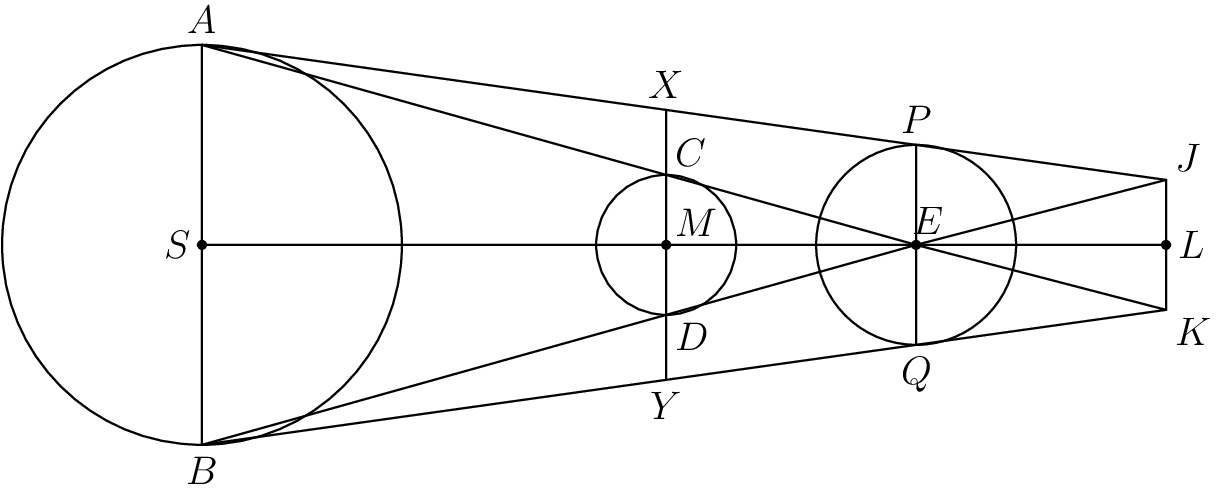
\includegraphics[scale=0.4]{img-hipparchus-2.png}
\end{figure}
In the diagram, points $S$, $M$, $E$, and $L$ lie on a line, with $S$, $M$, and $E$ representing the centers of the Sun, Moon, and Earth, respectively. Segments $\overline{AB}$, $\overline{CD}$, and $\overline{PQ}$ are diameters of their respective circles, all perpendicular to $\overline{SL}$. Segment $\overline{JK}$ is also perpendicular to $\overline{SL}$. Points $A, X, P, J$ are collinear, points $B, Y, Q, K$ are collinear, points $X, C, D, Y$ are collinear, points $A, C, E$ are collinear, and points $B, D, E$ are collinear. Finally, $E$ is the midpoint of $\overline{LM}$. Let $PE = 1$ (so lengths are in terms of Earth radii) and define
\begin{equation*}
\ell = EM = EL,\quad s = ES,\quad\theta = \angle CEM,\quad\phi = \angle JEL.
\end{equation*}
\begin{enumerate}
\item Show that 
\begin{equation*}
s = \frac{\ell}{(\tan\theta + \tan\phi)\ell - 1}
\end{equation*}
\item (Calculator recommended) The measurements used by Hipparchus were
\begin{equation*}
\ell\approx 67\tfrac{1}{3},\quad\theta\approx 0.277^{\circ},\quad\phi\approx 0.693^{\circ}.
\end{equation*}
Given these measurements, what value do we get for $s$?
\item (Calculator recommended) Currently, our measurements for the same quantities are
\begin{equation*}
\ell = 60.268,\quad\theta\approx 0.267^{\circ},\quad\phi\approx 0.746^{\circ}.
\end{equation*}
Given these measurements, what value do we get for $s$?\par
\end{enumerate}
\emph{Remark:} The true value of $s$ is $s\approx 23{,}455$, so some of the approximations made in order to set up the diagram turn out to be substantial sources of error.\newpage
\item A \emph{Pythagorean triple} is a triple $(X,Y,Z)$ of positive integers for which $X^2 + Y^2 = Z^2$. Note that if $(X,Y,Z)$ is a Pythagorean triple, then $(x,y) = (X/Z, Y/Z)$ is a point on the unit circle whose coordinates are rational numbers.
\begin{enumerate}
\item Let $O = (-1,0)$. If $P\neq O$ has rational coordinates and lies on the unit circle, then the slope of $\overline{OP}$ is rational. Conversely, show that if $\ell$ is a line passing through $O$ which has rational slope, then the other point $P\neq O$ at which $\ell$ intersects the unit circle must have rational coordinates.
\item Use part (a) to show that every point on the unit circle with rational coordinates can be written in the form $\displaystyle\left(\frac{n^2 - m^2}{n^2 + m^2}, \frac{2mn}{n^2 + m^2}\right)$ for integers $m$ and $n$.
\end{enumerate}
\emph{Remark:} A result going back to Euclid states that every \emph{primitive} Pythagorean triple, meaning a Pythagorean triple $(X,Y,Z)$ where $\gcd(X,Y,Z) = 1$, can be written as either
\begin{equation*}
X = n^2 - m^2,\quad Y = 2mn,\quad Z = n^2 + m^2
\end{equation*}
with $\gcd(m,n) = 1$ and $m + n$ odd, or in the same form with $X$ and $Y$ swapped.
\end{enumerate}


\newpage
\subsection{Answers}

\begin{enumerate}
\item \begin{enumerate}
\item $2\pi$ radians
\item $180^{\circ}$
\item $\pi/3$ radians
\item $135^{\circ}$
\item $\pi^2/900$ radians
\end{enumerate}
\item \begin{enumerate}
\item $\tan A = \frac{15}{8}$; $\cot A = \frac{8}{15}$
\item 17
\item $\sin A = \frac{15}{17}$; $\cos A = \frac{8}{17}$; $\sec A = \frac{17}{8}$; $\csc A = \frac{17}{15}$
\end{enumerate}
\item Since $\theta$ is acute, all six basic trig functions of $\theta$ have positive values.
\begin{enumerate}
\item Since $\sin^2\theta + \cos^2\theta = 1$, we know that $\cos^2\theta = \frac{8}{9}$, so $\cos\theta = \sqrt{\frac{8}{9}} = \frac{2\sqrt{2}}{3}$.
\item Since $\tan^2\theta + 1 = \sec^2\theta = 10$, we have $\tan\theta = 3$.
\item We build a right triangle $ABC$ with a right angle at $C$ and with leg lengths $AC = 5$ and $BC = 2$, so that $\tan\angle A = \frac{2}{5}$ and hence $\angle A = \theta$. Then, $AB = \sqrt{(AC)^2 + (BC)^2} = \sqrt{29}$ and $\csc\theta = \csc A = \frac{AB}{BC} = \frac{\sqrt{29}}{2}$.
\end{enumerate}
\item The completed table is below.
\begin{table}[H]
\centering
\begin{tabular}{c|c||c|c|c|c|c|c}
$\theta$ (deg) & $\theta$ (rad) & $\sin\theta$ & $\cos\theta$ & $\tan\theta$ & $\sec\theta$ & $\csc\theta$ & $\cot\theta$ \\ \hline
& & & & & & & \\
$30$ & $\frac{\pi}{6}$ & $\frac{1}{2}$ & $\frac{\sqrt{3}}{2}$ & $\frac{1}{\sqrt{3}}$ & $\frac{2}{\sqrt{3}}$ & $2$ & $\sqrt{3}$ \\
& & & & & & & \\ \hline
& & & & & & & \\
$45$ & $\frac{\pi}{4}$ & $\frac{1}{\sqrt{2}}$ & $\frac{1}{\sqrt{2}}$ & $1$ & $\sqrt{2}$ & $\sqrt{2}$ & $1$ \\
& & & & & & & \\ \hline
& & & & & & & \\
$60$ & $\frac{\pi}{3}$ & $\frac{\sqrt{3}}{2}$ & $\frac{1}{2}$ & $\sqrt{3}$ & $2$ & $\frac{2}{\sqrt{3}}$ & $\frac{1}{\sqrt{3}}$ \\
& & & & & & & 
\end{tabular}
\end{table}
\item \begin{enumerate}
\item 1
\item $1/2$
\item $-1/\sqrt{2}$
\item $\sqrt{3}/2$
\item $\sqrt{3}/2$
\item $-1/\sqrt{2}$
\end{enumerate}
\item \begin{enumerate}
\item $\sin\theta$
\item $-\cos\theta$
\item $-\sin\theta$
\item $-\cos\theta$
\item $-\sin\theta$
\item $\cos\theta$
\item $\cos\theta$
\item $\sin\theta$
\item $\cos\theta$
\item $-\sin\theta$
\end{enumerate}
\item \begin{enumerate}
\item We use the formula $[ABC] = \frac{1}{2}\cdot BA\cdot BC\cdot\sin B = 84$.
\item Let $D$ be the point on $\overline{BC}$ for which $\overline{AD}\perp\overline{BC}$. In right triangle $ABD$, we have that $AD = AB\sin B = 12$, so $BD = \sqrt{(AB)^2 - (AD)^2} = 5$. Then, $CD = BC - BD = 9$. (This is where we use the fact that the triangle is acute: it implies that $D$ is between $B$ and $C$.) Finally, $AC = \sqrt{(CD)^2 + (DA)^2} = 15$.
\item From $[ABC] = \frac{1}{2}\cdot AB\cdot AC\cdot\sin A$, we have $\sin A = \frac{2\cdot [ABC]}{AB\cdot AC} = \frac{56}{65}$.
\end{enumerate}
\item \begin{enumerate}
\item For $\chd 90^{\circ}$, we have $AB = \sqrt{(AO)^2 + (OB)^2} = \sqrt{2}$.\par
For $\chd 60^{\circ}$, note that triangle $AOB$ is equilateral, so $AB = 1$.\par 
For $\chd 30^{\circ}$, let $C$ be the point on $\overline{OB}$ for which $\overline{AC}\perp\overline{OB}$. Then $AC = \sin 30^{\circ} = \frac{1}{2}$ and $OC = \cos 30^{\circ} = \frac{\sqrt{3}}{2}$, so $BC = \frac{2 - \sqrt{3}}{2}$. The Pythagorean theorem gives
\begin{equation*}
AB = \sqrt{(AC)^2 + (CB)^2} = \sqrt{\frac{1}{4} + \frac{7 - 4\sqrt{3}}{4}} = \frac{\sqrt{8 - 4\sqrt{3}}}{2} = \frac{\sqrt{6} - \sqrt{2}}{2}.
\end{equation*}
\item Let $M$ be the foot of the perpendicular from $O$ to $\overline{AB}$. Since $OA = OB$, we have $MA = MB$ and $\angle AOM = \theta/2$, so $AB = 2(MA) = 2\sin(\theta/2)$.
\item Let $\overline{AC}$ be a diameter of a unit circle with center $O$ and let $B$ lie on the circle so that $\angle AOB = \theta$. Then $\angle BOC = 180^{\circ} - \theta$, so $AB = \chd\theta$ and $BC = \chd(180^{\circ} - \theta)$. As $\overline{AC}$ is a diameter, $\angle ABC = 90^{\circ}$. By the Pythagorean theorem,
\begin{equation*}
\chd^2\theta + \chd^2(180^{\circ} - \theta) = (AB)^2 + (BC)^2 = (AC)^2 = 4.
\end{equation*}
\end{enumerate}
\item \begin{enumerate}
\item Since $\overline{PE}$ is the midline of trapezoid $JLMX$, we have $JL + XM = 2(PE) = 2$. From right triangles $JLE$ and $CME$, we have $JL = \ell\tan\phi$ and $CM = \ell\tan\theta$, so $XC = 2 - \ell(\tan\theta + \tan\phi)$. Now, using the similarity $\triangle AXC\sim \triangle APE$,
\begin{equation*}
\frac{XC}{PE} = \frac{\text{height from \ensuremath{A} to \ensuremath{\overline{XC}}}}{\text{height from \ensuremath{A} to \ensuremath{\overline{PE}}}} = \frac{s - \ell}{s} = 1 - \frac{\ell}{s}.
\end{equation*}
Solving for $s$ gives the desired formula.
\item $s\approx 481.038$
\item $s\approx 918.779$
\end{enumerate}
\item \begin{enumerate}
\item Let $t$ be the slope of $\ell$, so the point-slope form of $\ell$ using $O$ as the reference point is $y = t(x + 1)$. Substituting this into $x^2 + y^2 = 1$, we get $x^2 + t^2(x + 1)^2 = 1$. Rearranging,
\begin{equation*}
(t^2 + 1)x^2 + 2t^2 x + (t^2 - 1) = 0.
\end{equation*}
We know that $x = -1$ is one solution (corresponding to point $O$), so the other solution, by Vieta's formula for the product, is $x = \frac{1 - t^2}{1 + t^2}$. Substituting this into the equation for $\ell$ gives $y = \frac{2t}{1 + t^2}$. When $t$ is rational, these coordinates are both rational.
\item In our result from the previous part, let $t = m/n$, where $m$ and $n$ are relatively prime, to get the desired form for any point $P\neq O$. For the point $O$ itself, let $n = 0$ and $m = 1$. (This corresponds to the vertical line $x = -1$ tangent to the unit circle at $O$.)
\end{enumerate}
\end{enumerate}